% This file was created by matplotlib v0.1.0.
% Copyright (c) 2010--2014, Nico Schlömer <nico.schloemer@gmail.com>
% All rights reserved.
% 
% The lastest updates can be retrieved from
% 
% https://github.com/nschloe/matplotlib2tikz
% 
% where you can also submit bug reports and leavecomments.
% 
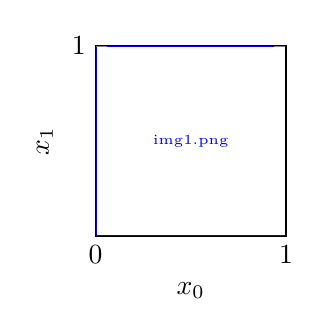
\begin{tikzpicture}

\begin{axis}[
xmin=0, xmax=1,
ymin=0, ymax=1,
axis on top,
width=4cm,
height=4cm,
% scaled x ticks=false,
xtick={0,1},
ytick={1},
% xticklabels={,,},
xlabel={$x_0$},
ylabel={$x_1$},
xlabel near ticks,
ylabel near ticks
]
\addplot graphics [includegraphics cmd=\pgfimage,xmin=0, xmax=1, ymin=0, ymax=1] {img1.png};
\path [draw=black, fill opacity=0] (axis cs:13,1)--(axis cs:13,1);

\path [draw=black, fill opacity=0] (axis cs:0.05,13)--(axis cs:0.05,13);

\path [draw=black, fill opacity=0] (axis cs:13,1.38777878078145e-17)--(axis cs:13,1.38777878078145e-17);

\path [draw=black, fill opacity=0] (axis cs:0,13)--(axis cs:0,13);

\end{axis}

\end{tikzpicture}
